% Created 2019-06-07 ven. 15:37
\documentclass[presentation]{beamer}
\usepackage[utf8]{inputenc}
\usepackage[T1]{fontenc}
\usepackage{fixltx2e}
\usepackage{graphicx}
\usepackage{longtable}
\usepackage{float}
\usepackage{wrapfig}
\usepackage{rotating}
\usepackage[normalem]{ulem}
\usepackage{amsmath}
\usepackage{textcomp}
\usepackage{marvosym}
\usepackage{wasysym}
\usepackage{amssymb}
\usepackage{hyperref}
\tolerance=1000
\usepackage[frenchb]{babel}
\setbeamertemplate{footline}{\leavevmode\hbox{\begin{beamercolorbox}[wd=.25\paperwidth,ht=2.25ex,dp=1ex,center]   {author in head/foot}\usebeamerfont{author in head/foot}\insertshortauthor\end{beamercolorbox}\begin{beamercolorbox}[wd=.50\paperwidth,ht=2.25ex,dp=1ex,center]{title in head/foot}\usebeamerfont{title in head/foot}\insertshorttitle\end{beamercolorbox}\begin{beamercolorbox}[wd=.25\paperwidth,ht=2.25ex,dp=1ex,right]{date in head/foot}\insertframenumber{} / \inserttotalframenumber\hspace*{2ex}\end{beamercolorbox}}\vskip0pt}
\AtBeginSection[]{\begin{frame}\vfill\centering\begin{beamercolorbox}[sep=8pt,center,shadow=true,rounded=true]{title}\usebeamerfont{title}\insertsectionhead\par\end{beamercolorbox}\vfill\end{frame}}
\usetheme{Singapore}
\usecolortheme{}
\usefonttheme{}
\useinnertheme{}
\useoutertheme{}
\author{Valentin Lebouvier}
\date{\today}
\title{TAL: Behaviour trees}
\hypersetup{
  pdfkeywords={},
  pdfsubject={},
  pdfcreator={Emacs 25.2.2 (Org mode 8.2.10)}}
\begin{document}

\maketitle


\section{Introduction}
\label{sec-1}
\begin{frame}[label=sec-1-0-1]{Sujet}
\alert{Projet IA en Python (part1): Behaviour tree et mission planning}
\end{frame}

\begin{frame}[label=sec-1-0-2]{Objectifs}
\begin{itemize}
\item Sujet 1 : Behaviour trees
\item Sujet 2 : Préparation TPs
\item Sujet 3 (optionnel): Mise en oeuvre sur du mission planning
\end{itemize}
\end{frame}

\begin{frame}[label=sec-1-0-3]{Plan}
\tableofcontents
\end{frame}


\section{Behaviour Trees}
\label{sec-2}
\begin{frame}[label=sec-2-0-1]{Behaviour Trees}
\begin{columns}
\begin{column}{0.5\textwidth}

\begin{itemize}
\item Outil de représentation de comportements permettant une modélisation et une implémentation simple ce ces comportements
\item Utilisé dans les domaines des jeux vidéos et de la robotique pour controller les comportements d'agents autonomes
\end{itemize}
\end{column}

\begin{column}{0.5\textwidth}
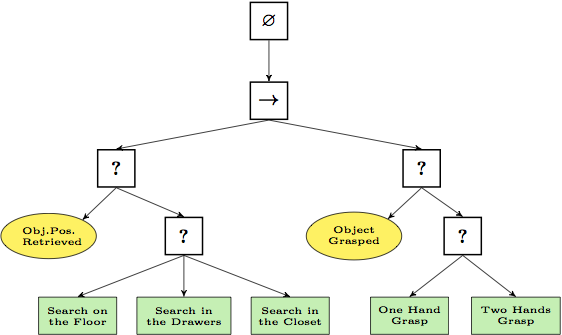
\includegraphics[width=.9\linewidth]{./img/BT_search_and_grasp.png}
\end{column}
\end{columns}
\end{frame}





\begin{frame}[label=sec-2-0-2]{Définition}
Un \alert{behaviour tree} (BT) est un graphe orienté acyclique dont chaque noeud retourne Succès (S), Échec (E) ou En Cours (R) selon les règles qui leurs sont associées.

L'évaluation d'un BT se fait par l'action d'un \emph{tick} sur son noeud racine, celui-ci évalue alors ses enfants de gauche a droite selon les règles qui sont associées a son type.

Les noeuds peuvent se trouver sous trois formes, les Composites, les Décorateurs et les noeuds d'Éxécution.
\end{frame}



\subsection{Décorateurs}
\label{sec-2-1}
\begin{frame}[label=sec-2-1-1]{Décorateurs}
\end{frame}

\subsection{Noeuds d'éxécution}
\label{sec-2-2}
\begin{frame}[label=sec-2-2-1]{\alert{Action}}
Représentation :

Retourne Succès si:
L'action s'est terminée correctement

Retourne Échec si:
L'action s'est mal terminée

Retourne En Cours si:
L'action est en cours
\end{frame}


\begin{frame}[label=sec-2-2-2]{\alert{Condition}}
Représentation :

Retourne Succès si:
La condition est vraie

Retourne Échec si:
La condition est fausse

Retourne En Cours si:
Jamais
\end{frame}

\subsection{Composites}
\label{sec-2-3}

\begin{frame}[label=sec-2-3-1]{\alert{Séquence}}
Représentation :

Retourne Succès si:
Tout les enfants ont réussis

Retourne Échec si:
Un enfant a échoué

Retourne En Cours si:
Un enfant est en cours
\end{frame}

\begin{frame}[label=sec-2-3-2]{\alert{Sélecteur}}
Représentation :

Retourne Succès si:
Un enfant a réussi

Retourne Échec si:
Tout les enfants ont échoués

Retourne En Cours si:
Un enfant est en cours
\end{frame}

\begin{frame}[label=sec-2-3-3]{\alert{Parallèle}}
Représentation :

Retourne Succès si:
M enfants ont réussis

Retourne Échec si:
F enfants ont échoués

Retourne En Cours si:
Aucun des précédents
\end{frame}

\begin{frame}[label=sec-2-3-4]{Composites avec mémoires}
\end{frame}


\section{PacMan}
\label{sec-3}
\begin{frame}[label=sec-3-0-1]{Frame 1}
\end{frame}


\section{TPs}
\label{sec-4}
\begin{frame}[label=sec-4-0-1]{Frame 1}
\end{frame}
% Emacs 25.2.2 (Org mode 8.2.10)
\end{document}